\documentclass[a4paper, 11pt]{article}
\usepackage{amsmath}
\usepackage{graphicx}
\usepackage{geometry}
\usepackage{listings}
\usepackage{xcolor}
\usepackage[colorlinks,linkcolor=red]{hyperref}
\geometry{scale=0.8}
\usepackage[UTF8]{ctex}
\title{	
\normalfont \normalsize
\textsc{School of Data and Computer Science, Sun Yat-sen University} \\ [25pt] %textsc small capital letters
\rule{\textwidth}{0.5pt} \\[0.4cm] % Thin top horizontal rule
\huge  E08 FF Planner(2)\\ % The assignment title
\rule{\textwidth}{2pt} \\[0.5cm] % Thick bottom horizontal rule
\author{18340052            何泽}
\date{\normalsize\today}
}

\begin{document}
\maketitle
\tableofcontents
\newpage

\section{Boxman Game}
If you don't know how to play the boxman game, you should open \texttt{BoxMan.zip} and click \texttt{BoxMan.exe} to have a try.  You can also choose the level of the game to challenge yourselves. There are five cases choosed from level 1, 10, 30, 40, 50 in the following figures.

You can model the location information based on rectangular coordinates as mapped out in Figure 3. For example, we denote by P13 the position (1,3). The calculated action sequence can be like this: \texttt{MOVE P12 P13, PUSH BOX1 P14 P15...},which means the guy runs from position (1,2) to position (1,3), and push the box1 from position (1,4) to position (1,5). However, this is only a very simple and intuitive approach to representing the actions and positions. If you have any other better methods, you can have a try.

Please solve the boxman game by using FF planner. You should hand in 2 files, including a domain file (\texttt{boxman\_domain.pddl}) and  data file (\texttt{boxman5.pddl}).
\begin{figure}[htb]
  \centering
  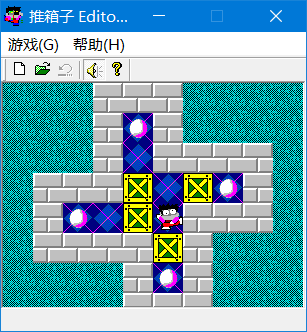
\includegraphics[width=4cm]{Pic/case1}
  \qquad
  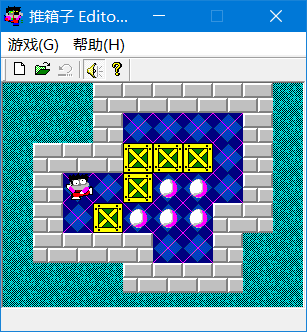
\includegraphics[width=4cm]{Pic/case2}
  \caption{Boxman case1 (level 1) and case2 (level 10)}
\end{figure}
\begin{figure}[htb]
  \centering
  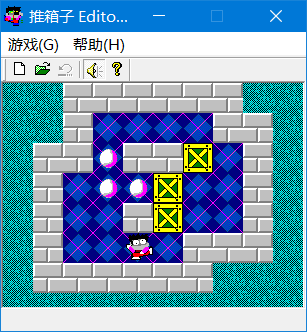
\includegraphics[width=4cm]{Pic/case3}
  \qquad
  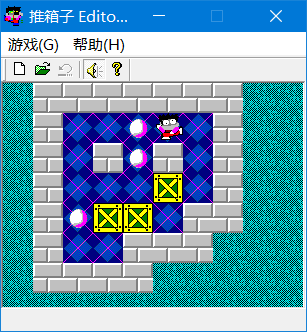
\includegraphics[width=4cm]{Pic/case4}
  \caption{Boxman case3 (level 30) and case4 (level 40)}
\end{figure}
\begin{figure}[htb]
  \centering
  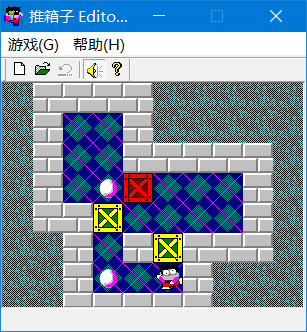
\includegraphics[width=4cm]{Pic/case5}
  \qquad
  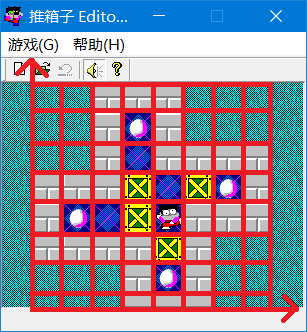
\includegraphics[width=4cm]{Pic/model}
  \caption{Boxman case5 (level 50) and modelling}
\end{figure}



\section{Notes}


\par Please send \textbf{E08\_YourNumber.zip} which should contain the codes(\textbf{ai\_2020@foxmail.com}). 

\section{Codes and Results}


My coordinate system:


\begin{figure}[htb]
\centering

\includegraphics[width=8cm]{Pic/2}

\caption{My model}
\end{figure}


\begin{lstlisting}[title=domain\_boxman.pddl,frame=single,language=lisp,numbers=left]
(define (problem prob)
    (:domain boxman)
    (:objects m b1 b2 b3 x1 x2 x3 x4 x5 x6 y1 y2 y3 y4 y5 y6 - physob)
    (:init  (man m)
        (position x1) (position y1) (position x2) (position y2)
        (position x3) (position y3) (position x4) (position y4)
        (position x5) (position y5) (position x6) (position y6)
        (blank x1 y1) (blank x1 y2) (blank x2 y1) (blank x2 y2)
        (blank x3 y1) (blank x3 y2) (blank x3 y4) (blank x3 y5) (blank x3 y6)
        (blank x4 y3) (blank x4 y4) (blank x4 y5) (blank x4 y6)
        (blank x5 y2) (blank x6 y2) (blank x6 y3)
        (add x1 x2) (add x2 x3) (add x3 x4) (add x4 x5) (add x5 x6)
        (add y1 y2) (add y2 y3) (add y3 y4) (add y4 y5) (add y5 y6)
        (sub x2 x1) (sub x3 x2) (sub x4 x3) (sub x5 x4) (sub x6 x5)
        (sub y2 y1) (sub y3 y2) (sub y4 y3) (sub y5 y4) (sub y6 y5)
        (box b1) (box b2) (box b3)
        (at  m x6 y4) (at b1 x3 y3) (at b2 x4 y2) (at b3 x5 y4)
        (capture x3 y3) (capture x4 y2) (capture x5 y4))
    (:goal (
         and (capture x3 y2) (capture x3 y3) (capture x6 y2)))
)
\end{lstlisting}

\begin{lstlisting}[title=boxman.pddl,frame=single,language=lisp,numbers=left]
(define (domain boxman)
    (:requirements
        :strips :equality :typing)
    (:types physob)
    (:predicates
        (blank ?x ?y - physob)(man ?x - physob) (box ?x - physob) 
        (target ?x ?y - physob) (capture ?x ?y - physob)
        (position ?x - physob) (at ?obj ?x ?y - physob) 
        (add ?new ?pre - physob) (sub ?new ?pre - physob)
    )
        
    (:action move_up
    :parameters (?m ?x ?y ?x_new - physob)
    :precondition (
        and (man ?m) (position ?x) (position ?y) (position ?x_new)
    	    (sub ?x ?x_new) (blank ?x_new ?y) (at ?m ?x ?y))
    :effect (
        and (not (blank ?x_new ?y)) (not (at ?m ?x ?y))
    	    (blank ?x ?y) (at ?m ?x_new ?y))
    )
    	    
    (:action move_down
    :parameters (?m ?x ?y ?x_new - physob)
    :precondition (
        and (man ?m) (position ?x) (position ?y) (position ?x_new)
    	    (add ?x ?x_new) (blank ?x_new ?y) (at ?m ?x ?y))
    :effect (and (not (blank ?x_new ?y)) (not (at ?m ?x ?y))
    	    (blank ?x ?y) (at ?m ?x_new ?y))
    )
    	   
    (:action move_left
    :parameters (?m ?x ?y ?y_new - physob)
    :precondition (
        and (man ?m) (position ?x) (position ?y) (position ?y_new)
    	    (sub ?y ?y_new) (blank ?x ?y_new) (at ?m ?x ?y))
    :effect (
        and (not (blank ?x ?y_new)) (not (at ?m ?x ?y))
            (blank ?x ?y) (at ?m ?x ?y_new))
    )
    
    (:action move_right
    :parameters (?m ?x ?y ?y_new - physob)
    :precondition (
        and (man ?m) (position ?x) (position ?y) (position ?y_new)
    	    (add ?y ?y_new) (blank ?x ?y_new) (at ?m ?x ?y))
    :effect (
        and (not (blank ?x ?y_new)) (not (at ?m ?x ?y))
            (blank ?x ?y) (at ?m ?x ?y_new))
    )

    (:action push_up
    :parameters (?m ?b ?x_man ?x ?y ?x_new - physob)
    :precondition (
        and (man ?m) (box ?b) (at ?m ?x_man ?y) (at ?b ?x ?y)
            (position ?x) (position ?y) (position ?x_new) (position ?x_man)
    	    (sub ?x_man ?x) (sub ?x ?x_new) (blank ?x_new ?y))
    :effect (
        and (not (blank ?x_new ?y)) (blank ?x_man ?y)
            (not (at ?b ?x ?y)) (not (at ?m ?x_man ?y))
            (at ?b ?x_new ?y) (at ?m ?x ?y)
            (capture ?x_new ?y) (not (capture ?x ?y)))
    )

    (:action push_down
    :parameters (?m ?b ?x_man ?x ?y ?x_new - physob)
    :precondition (
        and (man ?m) (box ?b) (at ?m ?x_man ?y) (at ?b ?x ?y)
            (position ?x) (position ?y) (position ?x_new) (position ?x_man)
    	    (add ?x_man ?x) (add ?x ?x_new) (blank ?x_new ?y))
    :effect (
        and (not (blank ?x_new ?y)) (blank ?x_man ?y)
            (not (at ?b ?x ?y)) (not (at ?m ?x_man ?y))
            (at ?b ?x_new ?y) (at ?m ?x ?y)
            (capture ?x_new ?y) (not (capture ?x ?y)))
    )
            
    (:action push_left
    :parameters (?m ?b ?y_man ?x ?y ?y_new - physob)
    :precondition (
        and (man ?m) (box ?b) (at ?m ?x ?y_man) (at ?b ?x ?y)
            (position ?x) (position ?y) (position ?y_new) (position ?y_man)
    	    (sub ?y_man ?y) (sub ?y ?y_new) (blank ?x ?y_new))
    :effect (
        and (not (blank ?x ?y_new)) (blank ?x ?y_man)
            (not (at ?b ?x ?y)) (not (at ?m ?x ?y_man))
            (at ?b ?x ?y_new) (at ?m ?x ?y)
            (capture ?x ?y_new) (not (capture ?x ?y)))
    )

    (:action push_right
    :parameters (?m ?b ?y_man ?x ?y ?y_new - physob)
    :precondition (
        and (man ?m) (box ?b) (at ?m ?x ?y_man) (at ?b ?x ?y)
            (position ?x) (position ?y) (position ?y_new) (position ?y_man)
    	    (add ?y_man ?y) (add ?y ?y_new) (blank ?x ?y_new))
    :effect (
        and (not (blank ?x ?y_new)) (blank ?x ?y_man)
            (not (at ?b ?x ?y)) (not (at ?m ?x ?y_man))
            (at ?b ?x ?y_new) (at ?m ?x ?y)
            (capture ?x ?y_new) (not (capture ?x ?y)))
    )
)

\end{lstlisting}

Results:

\begin{figure}[ht]
  \centering
  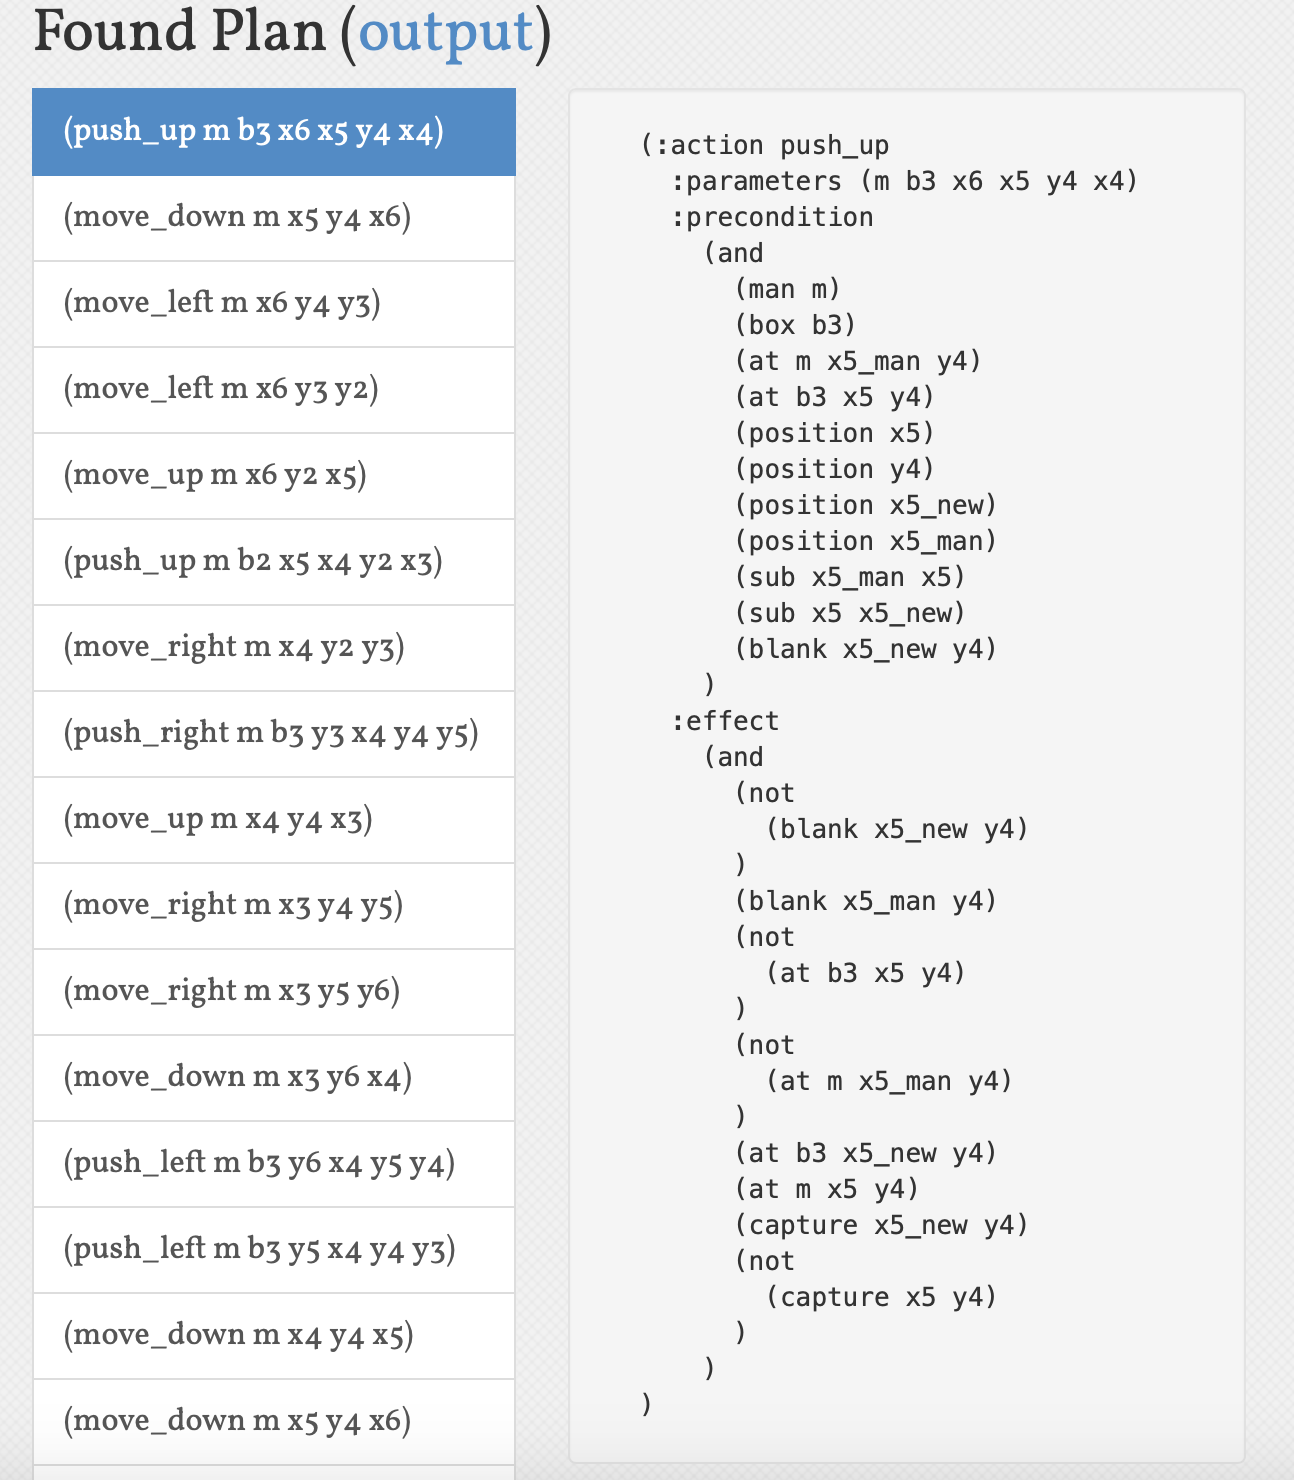
\includegraphics[width=0.9\textwidth]{Pic/1}
  \qquad
  \parbox[b]{0.6\textwidth}{Part of the result on the website\\}
\end{figure}
All results:
\begin{lstlisting}[title=result,frame=single,numbers=left]
(push_up m b3 x6 x5 y4 x4)
(move_down m x5 y4 x6)
(move_left m x6 y4 y3)
(move_left m x6 y3 y2)
(move_up m x6 y2 x5)
(push_up m b2 x5 x4 y2 x3)
(move_right m x4 y2 y3)
(push_right m b3 y3 x4 y4 y5)
(move_up m x4 y4 x3)
(move_right m x3 y4 y5)
(move_right m x3 y5 y6)
(move_down m x3 y6 x4)
(push_left m b3 y6 x4 y5 y4)
(push_left m b3 y5 x4 y4 y3)
(move_down m x4 y4 x5)
(move_down m x5 y4 x6)
(move_left m x6 y4 y3)
(move_left m x6 y3 y2)
(move_up m x6 y2 x5)
(move_up m x5 y2 x4)
(push_up m b2 x4 x3 y2 x2)
(push_right m b1 y2 x3 y3 y4)
(push_right m b1 y3 x3 y4 y5)
(move_down m x3 y4 x4)
(push_left m b3 y4 x4 y3 y2)
(move_up m x4 y3 x3)
(move_left m x3 y3 y2)
(push_down m b3 x3 x4 y2 x5)
(push_down m b3 x4 x5 y2 x6)
(move_up m x5 y2 x4)
(move_up m x4 y2 x3)
(move_right m x3 y2 y3)
(move_right m x3 y3 y4)
(move_down m x3 y4 x4)
(move_right m x4 y4 y5)
(move_right m x4 y5 y6)
(move_up m x4 y6 x3)
(push_left m b1 y6 x3 y5 y4)
(push_left m b1 y5 x3 y4 y3)
(move_down m x3 y4 x4)
(move_left m x4 y4 y3)
(move_left m x4 y3 y2)
(move_up m x4 y2 x3)
(move_left m x3 y2 y1)
(move_up m x3 y1 x2)
(move_up m x2 y1 x1)
(move_right m x1 y1 y2)
(push_down m b2 x1 x2 y2 x3)
\end{lstlisting}


%\clearpage
%\bibliography{E:/Papers/LiuLab}
%\bibliographystyle{apalike}
\end{document} 
%%% Local Variables:
%%% mode: latex
%%% TeX-master: t
%%% End:
